\chapter{Fundamentação Teórica}


\section{Sistemas de Controle}

Os sistemas de controle constituem um conjunto integrado de componentes que visam a regulação e a supervisão do
comportamento de sistemas dinâmicos.
Essenciais em uma muitas de aplicações práticas, são empregados para assegurar a estabilidade operacional e a precisão
de resposta a perturbações.
A operação desses sistemas pode ser realizada sob duas configurações principais: sistemas de malha aberta,
onde não há realimentação do estado do sistema, e sistemas de malha fechada, que se caracterizam pela incorporação de
realimentação na estratégia de controle.
A eficiência de um sistema de controle é determinada pela sua habilidade em alcançar e sustentar um estado operacional
desejado, reduzindo desvios e oscilações indesejadas.
A precisão com que um sistema de controle atinge e mantém a saída desejada, apesar das flutuações nos parâmetros ou nas
condições ambientais, é um indicador crítico de seu desempenho. \cite{ogata2010engenharia}.

Um sistema de controle em malha aberta opera sem a leitura de qualquer variável.
Nesse arranjo, o controlador atua baseado apenas no sinal de entrada, sem ajustar sua ação em resposta a distúrbios ou
variações na saída.
Um exemplo clássico é o controle de velocidade de um motor, onde a quantidade de combustível é ajustada apenas com base
na velocidade desejada, sem considerar a velocidade real do motor. \cite[Cap 2.3]{ogata2010engenharia}.

Em contraste, um sistema de controle em malha fechada inclui um ciclo de realimentação, onde a saída é continuamente
monitorada e comparada com o sinal de referência.
A diferença entre esses dois, conhecida como erro, é utilizada pelo controlador para ajustar o sinal de controle e,
assim, minimizar o erro. \cite[Cap 2.3]{ogata2010engenharia}.

    \begin{figure}[H]
    	\centering
    	\caption{Diagrama de blocos de um sistema de malha fechada}
    	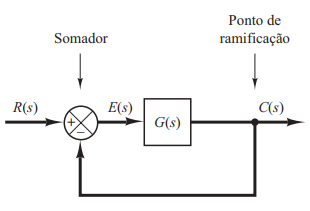
\includegraphics[scale=1]{figuras/closed_loop}
    	\label{fig:closed_loop}
    	\\
        \vspace{0cm}\hspace{0cm}\small{Fonte: \cite[Fig 2.3]{ogata2010engenharia}}
    \end{figure}

Onde:
\begin{itemize}
\item $R(s)$: Representa o sinal de referência.
\item $G(s)$: Representa o sistema sistema.
\item $C(s)$: Representa a saida.
\item $E(s)$: É o erro ou a diferença entre $R(s)$ e $C(s)$.
\end{itemize}

\subsection{Modelo}

De acordo com Coelho\cite{CoelhoIdentificacao}, em controle de processos, um modelo não busca ser uma réplica exata do
sistema real, mas sim uma representação adequada para uma aplicação específica.
A modelagem é um procedimento que visa obter um conjunto de equações matemáticas que descrevem a dinâmica do sistema,
permitindo responder a questões sobre o sistema sem a realização de experimentações físicas.
A simplicidade é muitas vezes uma virtude na modelagem de processos, pois modelos excessivamente complexos podem
não ser necessários para capturar a dinâmica essencial do sistema para fins de controle.

A função de transferência é uma forma comum de representar o modelo de um sistema em controle de processos.
Ela é definida como a razão entre a transformada de Laplace da saída e da entrada do sistema,
sendo uma razão de dois polinômios em $s$, onde $s$ é a variável complexa da transformada de Laplace.
Esta representação é particularmente útil para a análise e o projeto de sistemas de controle,
pois permite uma avaliação clara da resposta do sistema a diferentes tipos de sinais de entrada,
como impulso, degrau, rampa e senoidal.

Um modelo clássico e comumente utilizado para representação de sistemas de controle de primeira ordem com atraso é
representado pela seguinte função de transferência:
\begin{equation}
\label{eq:first_order_tf}
G(s) = \frac{K}{\tau s + 1}e^{-\theta s}
\end{equation}
onde cada termo tem um significado específico:
\begin{itemize}
\item $G(s)$: Função de transferência do sistema no domínio da frequência.
\item $K$: Ganho do sistema, que determina a amplitude da saída em relação à entrada.
\item $\tau$: Constante de tempo do sistema, que indica a rapidez com que o sistema responde a uma entrada.
\item $\theta$: Tempo de atraso, que representa o tempo que leva para a resposta do sistema começar após uma entrada.
\item $s$: Variável complexa da Transformada de Laplace, usada para transformar funções do tempo para o domínio da frequência.
\end{itemize}

Este modelo é particularmente útil para descrever sistemas onde há um atraso perceptível entre a ação de controle e a
resposta observada.
A exponencial negativa \( e^{-\theta s} \) incorpora o atraso no modelo, deslocando a resposta do sistema no tempo.
A constante de tempo \( \tau \) e o ganho \( K \) são parâmetros fundamentais que influenciam a dinâmica do sistema.
Através de simulações baseadas neste modelo, é possível prever o comportamento do sistema sob diferentes
condições operacionais e ajustar o projeto de um controlador antes da implementação real.

No contexto da automação industrial, os modelos matemáticos são empregados para previsão, análise e projeto de sistemas
de controle, essenciais para a sintonia de controladores e a otimização de processos.

\subsection{Controlador}

Dentro do universo dos sistemas de controle, um controlador é um componente crucial que modula a entrada de um sistema
para alcançar a saída desejada.
Ele atua ajustando o sinal de controle em resposta às variações da saída, visando minimizar a diferença entre a saída
observada e a saída desejada, conhecida como sinal de referência.
Os controladores podem ser classificados de acordo com suas ações de controle, alguns exemplos são controladores,
como on-off, proporcionais, integrais, proporcional-integrais (PI), proporcional-derivativos (PD) e
proporcional-integral-derivativos (PID), cada um com características distintas que os tornam adequados para diferentes
aplicações industriais. \cite[Cap 2.3]{ogata2010engenharia}.

%chck
O controlador PID é um dos tipos mais prevalentes de controladores em sistemas de controle, caracterizado pela sua
função de transferência,
\begin{equation}
\label{eq:ctrlr}
G_c(s) = K_p + \frac{K_i}{s} + K_d s
\end{equation}
onde \( K_p \), \( K_i \), e \( K_d \) representam os ganhos proporcional, integral e derivativo, respectivamente.
O termo proporcional \( K_p \) determina a reação do controlador à magnitude atual do erro,
o termo integral \( K_i \) acumula o erro ao longo do tempo, visando eliminar o erro estático,
e o termo derivativo \( K_d \) responde à taxa de variação do erro, antecipando o comportamento futuro.
A escolha adequada desses parâmetros é crucial: um \( K_p \) elevado pode acelerar a resposta do sistema, mas
potencialmente à custa da estabilidade;
um \( K_i \) excessivo pode introduzir oscilações devido ao atraso na resposta;
e um \( K_d \) significativo pode melhorar a estabilidade e a resposta rápida, mas é sensível ao ruído do sinal de
medição.
O ajuste dos três efeitos do controlador PID é essencial para otimizar o desempenho do sistema, tanto em resposta
transitória quanto em regime estacionário. \cite[Cap 2.3 e 8]{ogata2010engenharia}.

Vale ressaltar que controladores como P, PI e PD, podem ser vistos como um controlador PID onde o ganho para os
parâmetros não citados é ajustado para zero.

\subsection{Métodos de Identificação}

Fundamentação sobre Métodos de Identificação.

Um modelo bem construído permite a previsão dos estados futuros do sistema e a análise do comportamento dinâmico sob
perturbações atuantes.
A identificação e a modelagem de sistemas, portanto, constituem a base para a aplicação efetiva de técnicas de controle
em ambientes industriais.

\subsubsection{Ziegler Nichols}

Fundamentação sobre o método de identificação Ziegler Nichols

\subsubsection{Hagglund}

Fundamentação sobre o método de identificação Hagglund

\subsubsection{Smint}

Fundamentação sobre o método de identificação Smint

\subsubsection{Sundaresan Krishnaswamy}

Fundamentação sobre o método de identificação Sundaresan Krishnaswamy

\subsubsection{Nishikawa}

Fundamentação sobre o método de identificação Nishikawa

\subsection{Métodos de Aproximação de Controlador PID}

Fundamentação sobre Métodos de Aproximação de Controlador PID

\subsubsection{Ziegler Nichols}

Fundamentação sobre método de aproximação de ganhos Ziegler Nichols

\subsubsection{Cohen Coon}

Fundamentação sobre método de aproximação de ganhos Cohen Coon


\section{Software}

Introdução geral sobre controle teórica geral sobre controle

\subsection{Bibliotecas em Python}

Fundamentação Bibliotecas em Python

\subsection{Documentação de código}

Fundamentação Documentação de código

\subsection{Controle em Python}

Fundamentação Controle em Python

\subsection{Outras libs usadas}

Fundamentação Outras libs usadas


